\documentclass{article}
\usepackage[utf8]{inputenc}
\usepackage{graphicx}
\usepackage{float}
\usepackage{indentfirst}
\usepackage[portuguese]{babel}
\usepackage{biblatex}
\addbibresource{references.bib}

\title{IF680- Processamento Gráfico}
\author{Bruno de Figueiredo Lima}
\date{Dezembro, 2021}

\setlength{\parindent}{4em}

\begin{document}


\maketitle

\section{Introdução}
Processamento gráfico é a área que estuda processos ou técnicas computacionais que envolvem modelos geométricos e imagens digitais(ref). A partir dessa definição, nota-se que esse campo de estudo tem como referência principal a comunicação em seu aspecto visual, a qual é realizada através dos displays dos computadores e de seus dispositivos de interação\cite{foley1996computer}. Nesse sentido, tal disciplina não se resume apenas à produção de imagens de forma mecânica e descontextualizada, mas sim a interligação de conhecimentos de âmbitos de estudo distintos - como a matemática e seus conceitos de geometria e álgebra linear, a física e seus estudos do comportamento da luz, a biologia com seu foco no funcionamento da percepção visual humana e a engenharia através da elaboração de dispositivos que possam aperfeiçoar a produção de imagens - aplicados a tornar essa modalidade comunicação mais efetiva.

\section{Relevância}
A disciplina é de extrema relevância para os cursos de informática e, em especial, para a ciência da computação. Isso porque a visualização de informações é fundamental para que trabalhos de diferentes ramos de estudos dessas ciências sejam mais eficientes, principalmente aqueles que lidam com informações bastante complexas, como por exemplo o GPS e até mesmo o desenvolvimento de jogos eletrônicos. Dessa forma, conclui-se que a compreensão de processamento gráfico é uma ferramenta crucial para uma boa formação na área de informática.

\section{Relação com outras disciplinas}
A disciplina de Processamento Gráfico possui como pré-requisitos as disciplinas de Cálculo Diferencial e Integral 1 e Álgebra Vetorial e Linear para Computação, uma vez que variados conceitos destas são alicerces do estudo da área em questão. Mais à frente no curso, tal cadeira é pré-requisito de cadeiras como Computação Gráfica, já que o conhecimento de processamento gráfico é aprofundado nessa disciplina. 

\section{Aplicações}
Por trabalhar com a exibição de dados mediante o processamento de imagens, o Processamento Gráfico possui aplicações nas mais variadas áreas de conhecimento. Ele está presente em campos como a saúde, a educação, o entretenimento e a bioinformática\cite{WinNT}. A partir disso, pode-se apresentar de forma mais esclarecedora algumas dessas aplicações:

\begin{itemize}
    \item Saúde 
    
    Dentro dessa área, o processamento gráfico é mister para que a visualização de diagnósticos médicos, principalmente aqueles baseados em imagens como os de radiografia, sejam cada vez mais claros. 
    
    \begin{figure}[H]
        \centering
        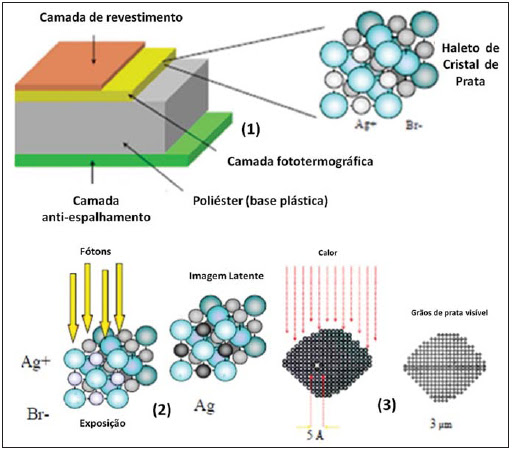
\includegraphics[width=68mm,scale=0.5]{images/radio.jpg}
        \caption{Representação esquemática dos diferentes níveis de profundidade de bits
esquema do processo de radiologia
 \cite{goto2013identificaccao}}
        \label{fig:esquema_radio}
    \end{figure}
    
    \begin{figure}[H]
        \centering
        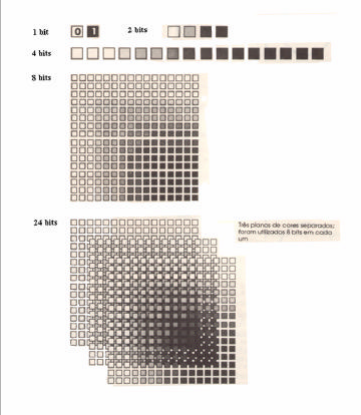
\includegraphics[width=42mm,scale=0.5]{images/bitradio.png}
        \caption{Representação de diferentes níveis de bits}
        \label{fig:bits}
    \end{figure}
    
    \item Entretenimento
    
    Em função do constante crescimento e progresso do mercado de jogos eletrônicos, o conhecimento de processamento gráfico é fundamental para o aperfeiçoamento dessa mídia. 
    
    \begin{figure}[H]
        \centering
        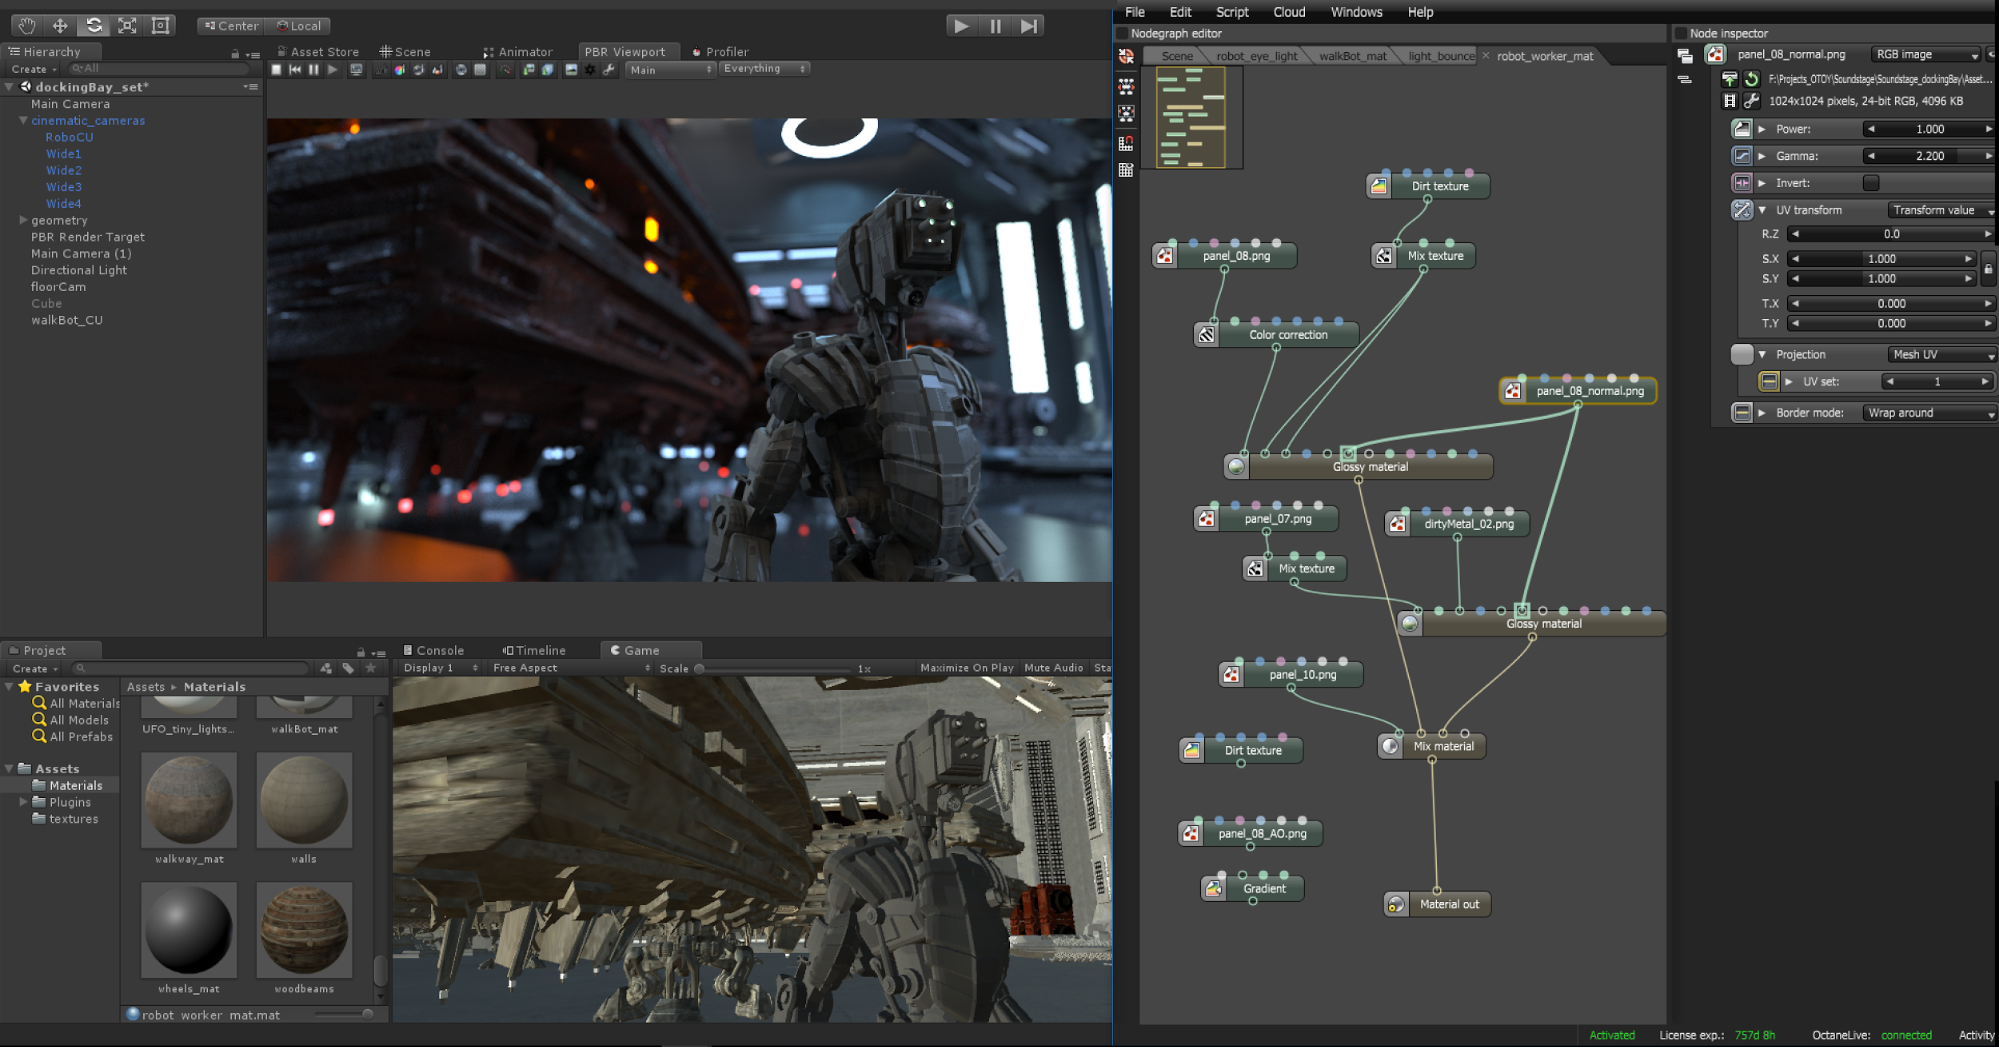
\includegraphics[width=100mm,scale=0.5]{images/pngegg.png}
        \caption{Processo de renderização no software Unity}
        \label{fig:render}
    \end{figure}
    
\end{itemize}

\printbibliography

\end{document}


